\documentclass[10pt,twocolumn]{article}
\usepackage[margin=0.75in,columnsep=0.25in]{geometry}
\usepackage[T1]{fontenc}
\usepackage{times}
\usepackage[authoryear,round]{natbib}
\usepackage{amsmath,amssymb}
\usepackage{graphicx}
\usepackage{booktabs}
\usepackage{xcolor}
\usepackage{hyperref}
\usepackage{url}
\graphicspath{{figures/}}
\makeatletter\let\tableinput\@@input\makeatother

\title{Power-State Variance in One WGPU Vector-Search Kernel:\\A Low-Cost Case Study with Qenlo}
\author{Akshat Singh Kushwaha \\ \texttt{akshatsingh14372@outlook.com}}

\date{}
\begin{document}
\makeatletter
\twocolumn[\@maketitle
\begin{center}\begin{minipage}{0.88\textwidth}\small\noindent\textbf{Abstract.} GPUs lower their clocks under light load, which is why careful kernel benchmarks lock clocks before timing. We measure what this does to a comparison between two GPU paths of one exact filtered vector-search engine, Qenlo, that return identical top-$k$ results. A \emph{light} path does device work proportional to the $E$ eligible rows; a deliberately naive \emph{heavy} path scans all $N$ rows and keeps the GPU at boost. Across fresh processes on an RTX 4050 Laptop GPU, RTX 4090s (one archived host and five cloud pods) and an H100, the heavy kernel's device time varied by at most 1\% between processes on one machine and 7\% across the five pods. The light kernel's varied up to $4.2\times$ on the laptop (at $E=3{,}000$) and $4.6\times$ across the pods; at $E=10{,}000$, where the light path beats our single-threaded CPU scan on the laptop and pods, the spreads were $1.4\times$ and $4.6\times$. On the laptop and H100, telemetry shows the driver running the light path at low clocks. On the laptop, in an experiment whose protocol was pushed before its data, locking the clocks removed the variation ($2.8\times$ to $1.00\times$ across blocks) and a low lock reproduced the slow mode, although one of five predictions failed; a second such experiment that locked the SM and memory clocks separately traced the selection kernel's slow mode mainly to the SM clock. Clocks could not be locked on the cloud hosts. There, a separate light GPU load made slow light-kernel runs rarer (clearly on the laptop, by a few runs on the pods and H100), but it also loaded the host, its planned end-to-end prediction failed, and sampled clocks did not track kernel time quantitatively, so the cross-host account is weaker. The cross-host comparison was exploratory. The magnitudes belong to this engine and these machines. The study ran on one laptop and about US\$6 of cloud time; protocols, raw data and telemetry are released.\end{minipage}\end{center}\vspace{1.2em}]
\makeatother
\thispagestyle{plain}

\section{Introduction}\label{sec:intro}
GPUs drop to lower clocks when they are lightly loaded. Kernel benchmarking practice knows this, and locks clocks or warms the device up before timing \citep{nvidia_ncu,nvidia_nvbench,nvidia_tensorrt_env}. Application-level benchmarks usually do neither. They compare implementations at the driver's default clocks, and the implementations being compared can load the GPU very differently. A work-efficient kernel that leaves the GPU mostly idle can be clocked down; a wasteful one that keeps it busy is not. The measured gap between them then partly reflects the power state each one induced. We report one case of this and test it.

The case comes from Qenlo, an embedded vector store with two GPU paths for exact filtered top-$k$ search that return identical results. A \emph{light} path uploads the list of $E$ eligible rows and does device work proportional to $E$. A \emph{heavy} path evaluates the filter inside the kernel and scans all $N$ rows; its selection kernel makes $k$ passes over all $N$ scores in one workgroup. The heavy path is not a competitive baseline. We keep it because it computes the same answer while holding the GPU at boost, which makes it a load contrast and a negative control. At $E=10{,}000$ eligible rows out of $N=100{,}000$, the light path is faster than both the heavy path and our single-threaded CPU scan on the laptop and the RTX 4090 pods (Appendix Table~\ref{tab:crossover}), so this is a regime where an application would choose it. (Part of that advantage comes from the CPU scan switching to slower FP64 accumulation above $E=4{,}096$; Section~\ref{sec:system}.) There its kernel time varied $1.4\times$ between fresh processes on the laptop and $4.6\times$ across five RTX 4090 cloud pods, while the heavy kernel's varied by at most 1\% on one machine and 7\% across the pods (Section~\ref{sec:repro}). At smaller $E$ the CPU wins and the light path's spread matters less in practice, although it is as large.

\begin{figure*}[t]
\centering
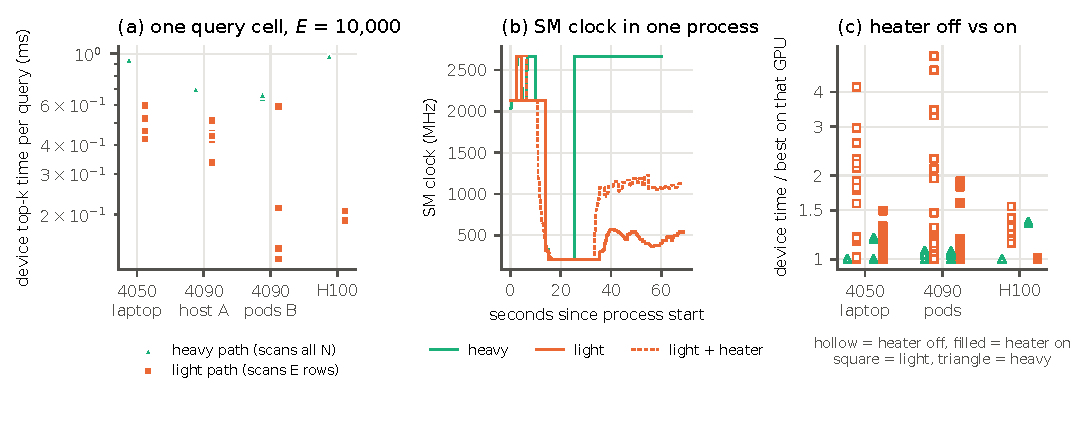
\includegraphics[width=\linewidth]{fig1_central.pdf}
\caption{\textbf{On the laptop, the light kernel's speed tracks the GPU clock.} (a) Device time of the top-$k$ kernel for one query cell ($N=100$K, $E=10{,}000$, $D=384$, $k=10$, batch~1), one point per fresh process. At this $E$ the light path is faster than the CPU scan on the laptop and pods (host A and the H100 had no CPU arm). The heavy path does $10\times$ more work and reproduces within 1\% on a machine and 7\% across the five RTX 4090 pods; the light path varies up to $1.5\times$ on a machine and $4.6\times$ across the pods. (b) SM clock sampled every 50\,ms during one laptop process per condition ($E=10{,}000$), including data loading. The heavy path stays at boost and the light path drops to about 500\,MHz; a separate light GPU load (the \emph{heater}) raises it to about 1.1\,GHz, still below boost. (c) Light (squares) and heavy (triangles) device time relative to the best value observed for that GPU and $E$, heater off (hollow) and on (filled), one point per block and $E$. With the heater, the light kernel's runs more than $1.5\times$ slow fall from 13 to 0 of 25 on the laptop, 7 to 4 of 25 on the pods and 1 to 0 of 9 on the H100, and the heavy kernel never gets faster.}
\label{fig:central}
\end{figure*}

The direct test is to lock the clock. That needs administrator rights, which we had on the laptop. There, in an experiment whose protocol and predictions were pushed to the public repository before its first run (Section~\ref{sec:lock}), locking the SM and memory clocks at boost removed the light kernel's spread across processes, and locking them at the light path's observed low state reproduced its slow mode. One of its five predictions failed: locked at boost, the light kernel took 32--50\% less time than the best unlocked median, outside the 15\% we had predicted.

Inside the cloud containers clocks could not be locked, so there we tried to raise the clock instead. A separate process, the \emph{heater}, keeps the GPU lightly busy. If the variation came only from contention, the heater could only slow every path down; if it came from power state, it should speed up work that was running below its attainable clock. At the device level that is the direction we saw on all three GPU types: light-kernel runs more than $1.5\times$ slower than their best fell from 13 of 25 to 0 on the laptop, 7 to 4 of 25 on the RTX 4090 pods and 1 to 0 of 9 on the H100, and the heavy kernel never got faster (Figure~\ref{fig:central}c, Section~\ref{sec:intervention}). The heater is a crude instrument. It also uses host CPU, it slowed host-side work by 40--48\% on the H100 pod at $E\le 3{,}000$, and the end-to-end speed-up we had planned to see did not appear on any GPU. Its protocols were written before the data but committed only afterwards (Appendix~\ref{app:protocols}). We treat the cross-host account as supported by telemetry and the heater, not as tested.

\paragraph{Why a small engine.} Everything here ran on one laptop plus about US\$6 of rented GPU time. That was possible because Qenlo is small enough to instrument end to end: device timestamps on every call, a fresh process per measurement, continuous clock telemetry, and two code paths with identical outputs that load the GPU differently. With those in place, finding the effect, testing it by locking clocks and releasing every sample took days. We think small, fully instrumented engines are a cheap way to do this kind of systems measurement, and we offer Qenlo as one.

\paragraph{Contributions.}
\begin{itemize}
\item \textbf{An observation in one engine.} For identical results, Qenlo's work-efficient GPU path is the less reproducible one. Its kernel time varies up to $4.2\times$ between fresh processes on the laptop (at $E=3{,}000$; $1.4\times$ at $E=10{,}000$) and $4.6\times$ across five same-model cloud hosts, while the heavy path's varies by at most 1\% on one machine and 7\% across those hosts (Section~\ref{sec:repro}).
\item \textbf{A locked-clock test on one laptop.} With its protocol committed before the data, locking the clocks removed the light kernel's variation and a low lock reproduced the slow mode. Locking the SM and memory clocks separately showed that the SM clock accounts for most of it; the memory clock matters only for the scoring kernel at the largest $E$ (Section~\ref{sec:lock}).
\item \textbf{Weaker evidence across hosts.} The heater's direction is consistent with the same account on RTX 4090 and H100 hosts, but sampled clocks do not track kernel time there quantitatively, and the planned end-to-end prediction failed; we report both (Sections~\ref{sec:states}--\ref{sec:intervention}).
\item \textbf{Reporting rules and data.} We consolidate existing rules for benchmarking latency-bound GPU work and add two (Section~\ref{sec:consequences}), and release protocols, raw samples, telemetry and hash manifests.
\end{itemize}

% Static sections (system, setup, related work). Included from main.tex.

\section{The query paths and why their load differs}\label{sec:system}
We study Qenlo, an embedded Rust vector store that answers exact (exhaustive) filtered cosine top-$k$ queries over a canonical collection of $N$ normalized FP32 vectors of dimension $D$ with per-row metadata. A predicate selects $E$ eligible rows; the query returns the $k$ eligible rows nearest to the query. Every execution path below returns the same result set (all runs pass an FP64-oracle recall@10 gate of 0.99; observed recall is 1.0 except where noted), so the choice of path affects only latency.

\paragraph{CPU scan.} A single-threaded AVX2 scan over the eligible rows. For $E\le 4{,}096$ it scores in FP32 and rescores boundary candidates in FP64; above that it accumulates in FP64 throughout. The kernel switch is part of the implementation and applies equally to every condition we compare.

\paragraph{GPU paths (WGPU/WGSL).} Vectors, identifiers and metadata are resident on the device. Each query uploads the query vector and an eligibility description, runs a scoring kernel and a top-$k$ selection kernel, and blocks on a readback of $k$ candidates, which the host merges. The paths differ only in how eligibility reaches the device:
\begin{itemize}
\item \emph{Compact rows (the light path).} The host materializes the sorted list of $E$ eligible row ids and uploads $4E$ bytes. Scoring and selection touch only those $E$ rows, so device work is proportional to $E$.
\item \emph{Shader predicate (the heavy path).} The host uploads per-row liveness ($4N$ bytes) and the predicate bounds; the kernels run over all $N$ rows and evaluate the predicate in the shader. Selection scans all $N$ scores $k$ times in one workgroup, so device work is proportional to $N$ regardless of $E$.
\end{itemize}
The heavy path therefore does up to $N/E$ times more device work for the same answer (1{,}000$\times$ at $E=100$, $N=10^5$). This selection kernel is deliberately simple and far from the best available; a tuned top-$k$ would narrow the gap. We use the heavy path as a load contrast and a negative control, not as a baseline: the two paths put very different loads on the GPU while computing identical results.

\paragraph{Timing boundary.} Latency is measured from the host search call to host-visible ordered results, including eligibility preparation, upload, dispatch, synchronization, readback and merge. Device-side scoring and selection times come from GPU timestamp queries in the same calls; they overlap host phases and are not additive. Host row materialization is timed separately on the CPU.

\section{Experimental design}\label{sec:setup}
\paragraph{Workload.} 100{,}000 AG News sentence embeddings (all-MiniLM-L12-v2, $D=384$; \citealp{nielsen2022agnews}) form the corpus; 5{,}000 disjoint held-out embeddings are the queries. Synthetic unique timestamps are attached to rows and a timestamp range selects exactly $E\in\{100, 1\text{K}, 3\text{K}, 10\text{K}, 30\text{K}\}$ eligible rows ($0.1\%$--$30\%$). Batch size is 1 and $k=10$, the regime of an interactive retrieval or agent-memory lookup.

\paragraph{Unit of replication.} Every condition runs in a fresh process: dataset load, 200 warm-up queries, then three passes over the 5{,}000 queries (15{,}000 timed calls). The per-process statistic is the lower median of the three per-pass percentiles. A \emph{block} runs every condition once in a shuffled order; blocks are the independent replicates. Paired effects are computed within a block and summarized by the median over blocks of per-block log-ratios, with 95\% percentile-bootstrap intervals over blocks (20{,}000 draws). With three to five blocks these intervals are coarse and we read them descriptively. The 15{,}000 calls within a process are repeated measurements and are never treated as independent.

\paragraph{Telemetry.} \texttt{nvidia-smi} samples SM clock, memory clock, performance state (P-state), utilization and power every 50\,ms for the whole life of each process. \texttt{nvidia-smi} itself observes the GPU only part of the time \citep{yang2023parttime}, so short kernels can fall between samples; we use the clocks to identify states, not to time kernels.

\paragraph{Intervention: a GPU heater.} To move the GPU's power state without touching the measured process, a separate process (the \emph{heater}) repeatedly dispatches a small compute kernel (64 workgroups $\times$ 256 threads, 500 dependent FMAs each), waits for it, and sleeps 1\,ms. Its own reported utilization is a few percent. On the GPU the heater can only compete with the measured process, so a speed-up it produces suggests that the measured process was held back by its power state and not by a lack of capacity. The heavy path, which already holds a high P-state, is the negative control. If contention were the only effect, the heater would slow both paths; if power state matters, it should speed up the light path and slow only the heavy one. The heater also uses host CPU, so it is not a clean GPU-only perturbation; its host cost shows up in end-to-end latency much more than in device timestamps (Section~\ref{sec:intervention}).

\paragraph{Hosts and protocols.} (i) A Windows~11 laptop (Intel i5-13420H, RTX 4050 Laptop GPU, driver 616.56, Vulkan, AC power, ``Balanced'' power plan). It uses hybrid graphics (Optimus); the display is driven by the Intel iGPU. (ii) RTX 4090s on Linux with Vulkan: \emph{host A}, an archive of five blocks on one host from September~24, and \emph{pods B}, five pods on five different hosts from September~25 with one block each. The pods use two driver branches (570.195 and 580.126--580.173). Because each pod ran one block, host and process variance are confounded on the pods. (iii) One H100 SXM pod (Linux, Vulkan) running a reduced design. A pod whose host CPU was about $14\times$ slower than the others was replaced before any of its results were inspected (Appendix~\ref{app:protocols}). The laptop, pod and H100 experiments (D1, D1R, H100) follow written protocols with predictions, but those were committed to version control only after the data; we call them planned analyses. The locked-clock protocol was committed and hashed before its first run. Clock locking (\texttt{nvidia-smi -lgc}) requires administrator rights; it was available on the laptop (Section~\ref{sec:lock}) and refused inside the cloud containers.



\section{Heavy kernels reproduce; light kernels do not}\label{sec:repro}
Table~\ref{tab:crosshost} reports the median device time of the top-$k$ selection kernel per fresh process, for both paths at three selectivities on four GPUs. We use device timestamps rather than end-to-end latency because they isolate the GPU from host-side effects; Section~\ref{sec:intervention} returns to end-to-end latency.

\begin{table}[t]\centering\small
\caption{Top-$k$ kernel device time per query (ms): median over fresh heater-off processes (min--max), and max/min across processes. Heavy = shader predicate over all $N=100$K rows; light = compact eligible rows. RTX 4090 host A is the retained September~24 archive (one host, 5 blocks); pods B are five September~25 pods on five different hosts, one block each. Identical binary source, dataset bytes and queries.}\label{tab:crosshost}
\begin{tabular}{rlrlrlr}\toprule
$E$ & GPU & $n$ & Heavy (ms) & max/min & Light (ms) & max/min \\\midrule
\tableinput{tables/cross_host}
\bottomrule\end{tabular}\end{table}

The heavy kernel reproduces within 1\% between processes on each single machine (the laptop, 4090 host A and the H100), and within 7\% across the five pod hosts, which span two driver branches (570 and 580). The light kernel does not. Its spread between processes reaches $2.6\times$ on 4090 host A, $4.2\times$ on the laptop and $4.3$--$4.6\times$ across the five 4090 pod hosts. At $E=3{,}000$ its median differs $3.8\times$ between host A and the pods (0.210 versus 0.055\,ms). The light path is still faster than the heavy path in every cell; what differs is how reproducible each path is.

The retained archive shows the same asymmetry within one host over time. Across ten identical blocks, the light path's selection time spans $2.44\times$ and correlates with the GPU clock recorded at process end (Spearman $\rho=-0.83$, $p=0.003$). The heavy kernels in the same archive vary by at most 0.1\% wherever their clock was at boost.

\section{Which power state each path gets}\label{sec:states}
Table~\ref{tab:states} reports the median SM and memory clocks while the GPU was active (samples with non-zero utilization) for each path. On every GPU the heavy path holds boost SM clocks: 2,670--2,820\,MHz on the consumer GPUs and 1,980\,MHz on the H100. The light path runs lower. At $E=10{,}000$ the driver also cuts the memory clock to 810\,MHz on the laptop (from 8,201\,MHz; performance state P5) and on the 4090 pods (from 10,501\,MHz). The scoring kernel reads every eligible vector, so a memory clock about $10\times$ lower can slow it substantially. On the H100 the light path's SM clock falls from 1,605 to 645\,MHz between $E=1{,}000$ and $10{,}000$.

\begin{table}[t]\centering\small
\caption{Median SM / memory clock (MHz) while the GPU is active, pooled over blocks. Clocks are sampled by \texttt{nvidia-smi} every 50\,ms, which is itself a partial sampler \citep{yang2023parttime}.}\label{tab:states}
\begin{tabular}{lrccc}\toprule
GPU & $E$ & Heavy path & Light path & Light path + heater \\\midrule
\tableinput{tables/power_states}
\bottomrule\end{tabular}\end{table}

We do not know what the governor responds to, so we state only what we observe. The heavy path spends 52--84\% of each call inside its two kernels and always holds boost. The light path spends 13--43\% and does not. Within the light path, however, the clock \emph{falls} as $E$ grows on the laptop and the H100, even though per-call device work grows. A simple busy-fraction account does not explain this. The busy fraction is also endogenous, because a lower clock lengthens the kernels that define it. The NVIDIA policy is undocumented \citep{spaan2026kerneldvfs}, and our claims concern its observable consequences.

\section{Intervention: making the GPU busier}\label{sec:intervention}
Each experiment ran every condition (engine $\times$ $E$ $\times$ heater on/off) once per block, in shuffled order and fresh processes (Section~\ref{sec:setup}). Table~\ref{tab:tail} gives the most direct test. For every block and $E$, it divides each path's device time by the best value observed for that GPU and $E$ in either arm. Both arms share the same reference, so a heater-off run that happened to be slow cannot flatter the heater through regression to the mean.

\begin{table}[t]\centering\small
\caption{Device time relative to the best observed for that GPU and $E$: median, 90th percentile, and share of runs more than $1.5\times$ slower than best, heater off versus on. One observation per block and $E$.}\label{tab:tail}
\begin{tabular}{llrcccccc}\toprule
& & & \multicolumn{3}{c}{Heater off} & \multicolumn{3}{c}{Heater on} \\\cmidrule(lr){4-6}\cmidrule(lr){7-9}
Path & GPU & $n$ & median & p90 & $>1.5\times$ & median & p90 & $>1.5\times$ \\\midrule
\tableinput{tables/tail}
\bottomrule\end{tabular}\end{table}

\paragraph{Device time: the predicted interaction appears on every GPU.} Without the heater, the light kernel runs a median 1.15--1.59$\times$ slower than its best, with a tail reaching $3.3\times$. With the heater, its median is 1.00--1.07; runs more than $1.5\times$ slow disappear on the laptop and the H100 and fall from 28\% to 16\% on the 4090 pods. The heavy kernel has no tail to remove. With the heater it becomes uniformly slower on the laptop ($1.19\times$) and the H100 ($1.36\times$), the cost of sharing the GPU, and stays unchanged on the 4090 pods. The heater's effect on the light kernel also grows with how slow that kernel was: across 59 block-level pairs, the heater-on/off ratio correlates with the heater-off slowdown (Spearman $\rho=-0.66$), and pairs that were at least $1.5\times$ slow were cut to a median 0.47. Unlike Table~\ref{tab:tail}, this correlation is exposed to regression to the mean, so we report it only as consistent with the account. Paired ratios with block-bootstrap intervals are in Appendix Table~\ref{tab:heater}.

\paragraph{End to end: small and host-dependent.} The heater also competes for GPU submission and readback, and on some hosts for the CPU: on the H100 pod it slowed host row materialization by 40--48\%. End to end, the light path's median call latency with the heater was 0.94--0.96 of its heater-off value on the 4090 pods at $E=3{,}000$--$10{,}000$ (1.07 at 30{,}000) and 0.95--0.97 on the laptop at $E\ge 3{,}000$, with intervals that mostly include 1. On the H100 it was 1.10--1.24. Heavy calls were 6--9\% slower on the consumer GPUs and 25--27\% slower on the H100. Under the same added load the light path fared better than the heavy path in 10 of 13 cells, but whether it gained or lost overall depends on how much contention the host adds. The $1.9\times$ end-to-end speed-up in our laptop pilot did not replicate reliably across blocks.

\paragraph{Scorecard against the preregistered predictions (Appendix Table~\ref{tab:scorecard}).}
\begin{itemize}
\item P1 predicted a light-path end-to-end speed-up of at least 10\% at $E\le 3{,}000$. It \emph{failed} on every GPU.
\item P2 predicted no heavy-path speed-up. It held in every cell.
\item P3 predicted that the light path's ratio would fall below the heavy path's. It held in every cell for device time and in 10 of 13 cells end to end.
\item P4 predicted that light device time falls while host materialization stays within 10\%. It held in 6 of 13 cells and failed where the heater also slowed the host.
\end{itemize}
The device-level predictions, which isolate the GPU, held; the end-to-end prediction did not.

\section{Consequences}\label{sec:consequences}
\paragraph{Unlocked-clock benchmarks can understate the efficient implementation.} A benchmark that compares a work-efficient GPU kernel with a less efficient one at low load runs the efficient one at a lower clock. Here the light path won every cell regardless. But its measured device-time advantage over the heavy path at $E=3{,}000$ is $3.4\times$ on 4090 host A, $9.0\times$ on the laptop, $10.5\times$ on the H100 and $12.6\times$ on the 4090 pods, for identical code. Optimizations that remove GPU work (tighter filtering, smaller kernels, early exit) can be measured at a discount the benchmark does not show, and the discount differs between machines.

\paragraph{Kernel-level results did not transfer between machines with the same GPU.} Six RTX 4090 hosts gave light-kernel medians spanning $3.8\times$ for the same cell. Any threshold or cost model calibrated on one of them, for example a CPU/GPU router, partly encodes that host's power behavior. The study that preceded this one fitted a scalar CPU/GPU routing threshold with zero errors on 31 development pairs. On a preregistered held-out suite it chose the slower route in 8 of 16 workloads, several of them within the process-to-process variation measured here (Appendix~\ref{app:router}). In our data the heater never changed a CPU/GPU winner (Appendix Table~\ref{tab:crossover}). We therefore do not claim that power state moves this system's crossover, only that it moves the margins a router is calibrated on.

\paragraph{Isolated benchmarks may misstate co-located latency.} In deployment a retrieval kernel often shares the GPU with a model; our heater is a crude stand-in for that load. On an idle GPU the light path is exposed to deep power states; under load, to contention. The heavy path is exposed only to contention. Latency measured on an idle GPU is therefore a poor proxy for latency under co-location, and the error can differ between implementations. We did not test co-location with a real model.

\paragraph{What to report.} For latency-bound GPU work:
\begin{enumerate}
\item[(i)] Replicate across fresh processes and report the spread between them; repetitions inside one process share its power state.
\item[(ii)] Log clocks and performance state continuously, not just before and after a run.
\item[(iii)] Report device-timestamp kernel time alongside end-to-end latency, to separate power-state effects from host effects.
\item[(iv)] Where clocks cannot be locked, add a load-raising control such as the heater, together with a heavy negative control.
\item[(v)] When comparing implementations, state whether they ran in the same power state.
\end{enumerate}


\section{Related work}\label{sec:related}
\paragraph{Power management versus latency.} On servers, low-power states and slow frequency governors are known to inflate the latency of latency-critical services at low load \citep{meisner2011powermgmt,kanev2014tradeoffs}, motivating latency-aware controllers \citep{lo2014pegasus,kasture2015rubik,hsu2015adrenaline,chou2019mudpm}. Mobile GPU governors mispredict bursty and concurrent work \citep{pathania2014integrated,lin2023geardvfs,zhang2025mobiledvfs}, and at low locked clocks desktop GPUs can drop into idle-like states \citep{adamek2021fftedge}. GPU DVFS work for machine learning treats frequency as a knob to \emph{lower} for energy \citep{tang2019gpudvfsdl,you2023zeus,chung2024perseus,qiu2024muserve,stojkovic2025dynamollm,kakolyris2025throttllem,maliakel2025llmdvfs,spaan2026kerneldvfs}. We study the opposite case, in which the default policy under-clocks latency-bound work that the application would prefer to run fast. We have not found a report that this changes the measured margin between two implementations of the same GPU operation, or that an unrelated co-running GPU load speeds up a latency-bound GPU kernel.

\paragraph{Benchmark validity.} Innocuous setup details bias measured speed-ups \citep{mytkowicz2009wrongdata}; variation across executions must be sampled and reported \citep{kalibera2013rigorous,maricq2018taming}. For GPUs, power management causes 8--22\% variation across same-model devices under load \citep{sinha2022notallgpus} and 1--14\% in GEMM timings \citep{golden2025prism}; kernel benchmarking practice therefore often locks clocks \citep{oliaro2026fastkernels,chu2026operatorprofiler}, and \texttt{nvidia-smi} telemetry itself is sampled only part-time \citep{yang2023parttime}. The variation we measure is much larger (up to $4.6\times$ rather than tens of percent), and it makes the less efficient implementation look relatively better.

\paragraph{Filtered vector search and CPU/GPU placement.} Filtered nearest-neighbor search is an active area \citep{gollapudi2023filtered,patel2024acorn,iff2026fanns,shi2025unified,li2025attribute,amanbayev2026systems}, including GPU systems \citep{johnson2019billion,xi2025vecflow}. Whether to run vector search on a GPU at all depends on data movement and batch size \citep{gregg2011whereisdata,mageirakos2026togpu}, and cost-model-based CPU/GPU operator placement is known to be fragile \citep{bress2016robust}. The choice between an eligible-id list and a full-width filter mirrors selection vectors versus bitmaps in vectorized databases \citep{ngom2021filter}. We add that the measured margins between such alternatives can depend on the GPU's power state, which the alternatives themselves influence.


\section{Limitations}\label{sec:limitations}
\emph{One engine, one kernel pair.} Both paths come from Qenlo, with a simple hand-written WGSL selection kernel, and the heavy path is deliberately naive. Tuned library kernels such as FAISS or cuVS may load the GPU differently and run in different states; testing them, and more hosts per GPU model, needs compute we did not have. We do not expect these magnitudes to carry over. \emph{Clock locking on one machine.} Locking was possible only on the laptop and was refused in the cloud containers, so the cross-host account rests on telemetry and the heater, which also loads the host. The locked-clock test covers one GPU, one driver and one operating system. \emph{Laptop platform.} The laptop uses hybrid graphics (Optimus): the display runs on the Intel iGPU and the RTX 4050 renders nothing else during the runs. It ran on AC power under the Windows ``Balanced'' plan; we did not test other plans. \emph{Telemetry.} \texttt{nvidia-smi} samples every 50\,ms; clocks are reported for active samples of a whole process, including warm-up, so they cannot show the clock during a sub-millisecond kernel. We did not record clock-event reasons or the NVIDIA power-management mode, and we did not test whether ``prefer maximum performance'' (which needs no administrator rights) reproduces the lock. \emph{Timestamps.} Device times come from pass-level timestamp queries, so after an idle gap they may include wake-up latency as well as slower execution. \emph{Drift.} The laptop's unlocked behavior changed between D1 and E-LOCK (Section~\ref{sec:lock}). \emph{CPU baseline.} The CPU scan is single-threaded and switches to FP64 above $E=4{,}096$; a stronger CPU path could move the crossover. \emph{Small $n$ and confounding.} Five blocks on the laptop, five RTX 4090 pods with one block each on five different hosts, and three H100 blocks. On the pods, host and process variance cannot be separated, and with three to five blocks the bootstrap intervals are block ranges, not 95\% intervals. About 65 cell-level verdicts were scored without multiplicity control. The pods also span two driver branches. One pod was replaced before analysis because its host CPU was about $14\times$ slower on a single-threaded test; its partial block is archived but excluded. \emph{Host coupling.} On the laptop and the H100 the heater also changed host-side timings, so end-to-end effects there cannot be attributed to the GPU clock alone. \emph{API.} All runs use Vulkan through WGPU; CUDA runtimes may be managed differently. \emph{Driver versions.} 616.56 (Windows) and 570.195--580.173 (Linux).

\section{Conclusion}\label{sec:conclusion}
In Qenlo, the faster GPU path for a light query was also the one whose kernel time varied most between processes and machines. On the laptop the variation tracked the clock the driver chose, and fixing the clock removed it. On the cloud hosts we could only raise the GPU's load, which made the light kernel's slow runs rarer at the device level but did not make calls faster end to end. On the laptop the heavy path held a high clock, so it looked more stable than it would at equal clocks, and its gap to the light path looked smaller ($2.0\times$ unlocked against $8.3\times$ locked at $E=10{,}000$). For benchmarks of light GPU work, we would record the power state, replicate across fresh processes, and report device time separately from end-to-end latency. A small engine with this much instrumentation can test whether similar effects appear in other kernels for little money, which is the use we have in mind for it.

\section*{Reproducibility}
Each experiment's protocol and predictions were written before its data were collected, by our records, but only the two locked-clock protocols (E-LOCK and E-SPLIT) were pushed to the public repository before their data; GitHub's push times show the order (Appendix~\ref{app:protocols}). The others were committed the same evening, after collection. Every raw archive and the E-LOCK/E-SPLIT trees have SHA-256 manifests, and the runner logs are committed. Raw per-call samples, 50\,ms telemetry, analysis scripts and the heater are in the repository: \path{research/data/raw/2026-09-25-dvfs-*}, \path{research/scripts/analyze_dvfs_d1.py}, \path{research/scripts/cross_host.py}, \path{research/scripts/pool_hosts.py} and \path{crates/qenlo/examples/gpu_heater.rs}. Tables~\ref{tab:crosshost}, \ref{tab:states} and \ref{tab:scorecard}--\ref{tab:crossover} come from \path{paper/v2/scripts/make_tables.py} over CSVs that \path{research/scripts/cross_host.py} and \path{pool_hosts.py} produce from the extracted archives; Tables~\ref{tab:tail}, \ref{tab:lock} and \ref{tab:split} come from \path{tail_table.py}, \path{analyze_dvfs_lock.py} and \path{analyze_dvfs_split.py}. An independent re-implementation by an outside audit reproduced every table cell. Cloud compute for the new runs cost about US\$6.

\bibliography{references}
\bibliographystyle{plainnat}

\appendix
\section{Protocols, predictions and deviations}\label{app:protocols}
Four protocols were written and SHA-256 hashed before their data existed: the laptop experiment D1 (\path{research/experiments/dvfs-d1/protocol.md}), the RTX 4090 pod replication D1R (\path{dvfs-d1r/}), the H100 arm (\path{dvfs-h100/}) and an API/batch follow-up D2 (\path{dvfs-d2/}, not yet run). A fifth, the locked-clock experiment E-LOCK (\path{research/experiments/dvfs-lock/}), was hashed on 2026-10-19 before its data and ran on the laptop only. One exploratory pilot preceded them (\path{research/data/raw/2026-09-25-dvfs-pilot/}) and is used only to motivate the design. D1 predicted, for batch-1 queries:
P1, the heater lowers light-path end-to-end P50 by at least 10\% (ratio $<0.9$, interval excluding 1) at $E\le 3{,}000$;
P2, the heater does not speed up the heavy path (ratio $\ge 0.95$);
P3, the light path's ratio is below the heavy path's;
P4, the heater lowers light-path device time while host row materialization stays within $\pm10\%$.
The same rules were applied unchanged to every host.

\begin{table}[h]\centering\footnotesize
\caption{Preregistered predictions by GPU and $E$. P3 is shown for end-to-end P50 / device time. ``n/a'': P1 was registered only for $E\le 3{,}000$.}\label{tab:scorecard}
\setlength{\tabcolsep}{4pt}\begin{tabular}{lrcccc}\toprule
GPU & $E$ & P1 call $<0.9$ & P2 heavy $\ge 0.95$ & P3 light $<$ heavy & P4 device $\downarrow$, host flat \\\midrule
\tableinput{tables/scorecard}
\bottomrule\end{tabular}\end{table}

P1 fails everywhere at the block level; the pilot's $1.9\times$ end-to-end speed-up on the laptop did not replicate reliably across blocks. P2 and the device-time half of P3 hold in every cell. P4 fails where the heater also slowed host-side work. On the H100 pod, host row materialization became 40--48\% slower with the heater running, which shows that the heater process took host CPU time as well as GPU time. The end-to-end slowdowns on that host therefore say little about the power-state account; they show that our heater is not a clean GPU-only perturbation.


\begin{table}[h]\centering\scriptsize
\caption{Paired heater-on / heater-off ratios (median over blocks of per-block ratios, 95\% block-bootstrap interval). Below 1 = faster with the heater. Device = top-$k$ kernel time; call = end-to-end P50. $n$ = blocks.}\label{tab:heater}
\begin{tabular}{lrrllll}\toprule
GPU & $E$ & $n$ & Light device & Heavy device & Light call & Heavy call \\\midrule
\tableinput{tables/heater_effects}
\bottomrule\end{tabular}\end{table}

\paragraph{Deviations.} (i) The clock summary in the preregistered analysis script took the median over the whole process, including data loading; we added a GPU-active median (utilization $>0$) before inspecting any cross-host comparison and report both in the released CSVs. (ii) Two pod setup attempts failed because of script bugs (a missing dataset copy, a mis-specified pod) and were re-run before any cell completed; no completed cell was discarded. (iii) The pod first assigned to block~3 ran host-side benchmark work roughly $10\times$ slower than the others (about $14\times$ on a single-threaded Python test). Before any of its results were inspected, we re-ran block~3 from scratch on a new pod (Ryzen~9 7950X). The 14 cells the slow pod completed are retained (\path{d1r-b3-partial.tar.gz}) and excluded from the tables. A stray setup process ran for about 30\,s on the block~4 pod during three cells; dropping those cells changes the affected light-path ratio from 0.967 to 0.966. (iv) The cross-host table (Table~\ref{tab:crosshost}) and the device-time framing were not preregistered; they were suggested by the retained September~24 archive and are therefore partly exploratory, although the pods and H100 supplied new data for them.

\paragraph{E-LOCK predictions.} K1 (light max/min $\le 1.15$ locked high), K3 (locked-low light time within 25\% of D1's slow mode at $E=10{,}000$), K4 (no heater effect locked high) and K5 (heavy within 3\% of unlocked) held in every tested cell. K2 (locked-high light time within 15\% of the best unlocked) failed as written, because locked-high was 32--50\% \emph{faster} than the best unlocked median. No run was excluded and the run followed the protocol, with memory clocks locked as planned. Analysis: \path{research/scripts/analyze_dvfs_lock.py}.

\section{CPU/GPU crossover}\label{app:crossover}
\begin{table}[h]\centering\small
\caption{Median-block end-to-end P50 (ms) for the single-threaded CPU scan, the light GPU path with the heater off and on (winner against CPU in parentheses), and the heavy GPU path. The heater never changed a winner.}\label{tab:crossover}
\begin{tabular}{lrrllr}\toprule
GPU & $E$ & CPU & Light, heater off & Light, heater on & Heavy \\\midrule
\tableinput{tables/crossover}
\bottomrule\end{tabular}\end{table}

\section{The held-out router failure that motivated this study}\label{app:router}
The system's earlier research campaign (preserved unchanged in \path{paper/paper.tex}) selected a scalar routing rule, GPU if $E\cdot D\cdot B\ge 10^6$, with zero errors on 31 development CPU/GPU pairs. On a preregistered held-out suite of 16 workloads on an RTX 4050 laptop it chose the slower route in 8, with median regret 0.4\% and maximum regret 235.7\%. Each route was measured in a single process with five in-process runs. An audit of that archive found that the automatic arm differed from the forced arm of the same backend by more than 25\% in 9 of 16 cells, and that two of the eight ``wrong'' labels were within 3.2\% regret. In light of Section~\ref{sec:repro}, labels near parity in such a suite partly measure the GPU's power state during each process, and the per-workload count is not a stable statistic. The maximum-regret rejection survives: a $3.36\times$ ratio exceeds every within-host spread we measured except the laptop light path's $4.2\times$. The earlier manuscript also documents representation, preparation and harness findings that are not repeated here.

\section{Cost and resources}
New cloud runs used five RTX 4090 pods (one block each), one H100 SXM pod and a 4-minute H100 probe, at \$0.74 and \$3.49 per hour. The operator's ledger totals about US\$6 (\path{research/experiments/dvfs-d1r/campaign-log.md}). All pods were deleted after their data were downloaded and hash-checked. A container-level Vulkan fix (pointing the loader at \texttt{libEGL\_nvidia.so.0} rather than the toolkit's GLX ICD) was required on every pod and is documented in the log; it may explain an earlier ``no Vulkan'' failure on an A6000.

\end{document}
